% book example for classicthesis.sty
\documentclass[10pt,paper=a4 BCOR0, DIV15]{scrbook} % KOMA-Script book
\usepackage[T1]{fontenc}                
\usepackage{lipsum}
\usepackage[linedheaders,parts,pdfspacing]{classicthesis} % ,manychapters
%\usepackage[osf]{libertine}
\usepackage{amsthm}
\usepackage[T1]{fontenc}
\usepackage[utf8]{inputenc}
\usepackage{polski}
\usepackage{hyperref}
\usepackage{graphicx}
\usepackage{geometry}
%\newgeometry{tmargin=2.5cm, bmargin=1.5cm, lmargin=1.5cm, rmargin=1.5cm}
\urlstyle{sf} 
\renewcommand{\contentsname}{Instrukcja obsługi programu Mopnik}
\begin{document}
%	\pagestyle{scrheadings}
%	\manualmark
%	\markboth{\spacedlowsmallcaps{\contentsname}}{\spacedlowsmallcaps{\contentsname}}
	
	\tableofcontents 

%	\automark[section]{chapter}
%	\renewcommand{\chaptermark}[1]{\markboth{\spacedlowsmallcaps{#1}}{\spacedlowsmallcaps{#1}}}
%	\renewcommand{\sectionmark}[1]{\markright{\thesection\enspace\spacedlowsmallcaps{#1}}}

    % use \cleardoublepage here to avoid problems with pdfbookmark
    %\cleardoublepage\part{Widok po uruchomieniu programu}
    \chapter{Widok po uruchomieniu programu}
    %\addtocounter{chapter}{1}
    \section{Wyświetlanie mapy}
    \paragraph{}
    Po uruchomieniu programu ładowane są domyślne dane:
    \begin{enumerate}
    \item Kafelki mapy w formacie graficznym (służą one tylko wizualizacji).
    \item Mapa sieci drogowej w formacie OSM.
    \item Dane dotyczące średniodobowego natężenia ruchu.
    \item Dane dotyczące rozmieszczenia MOP-ów.
    \end{enumerate}
 \begin{figure}[ht]
      \centering
      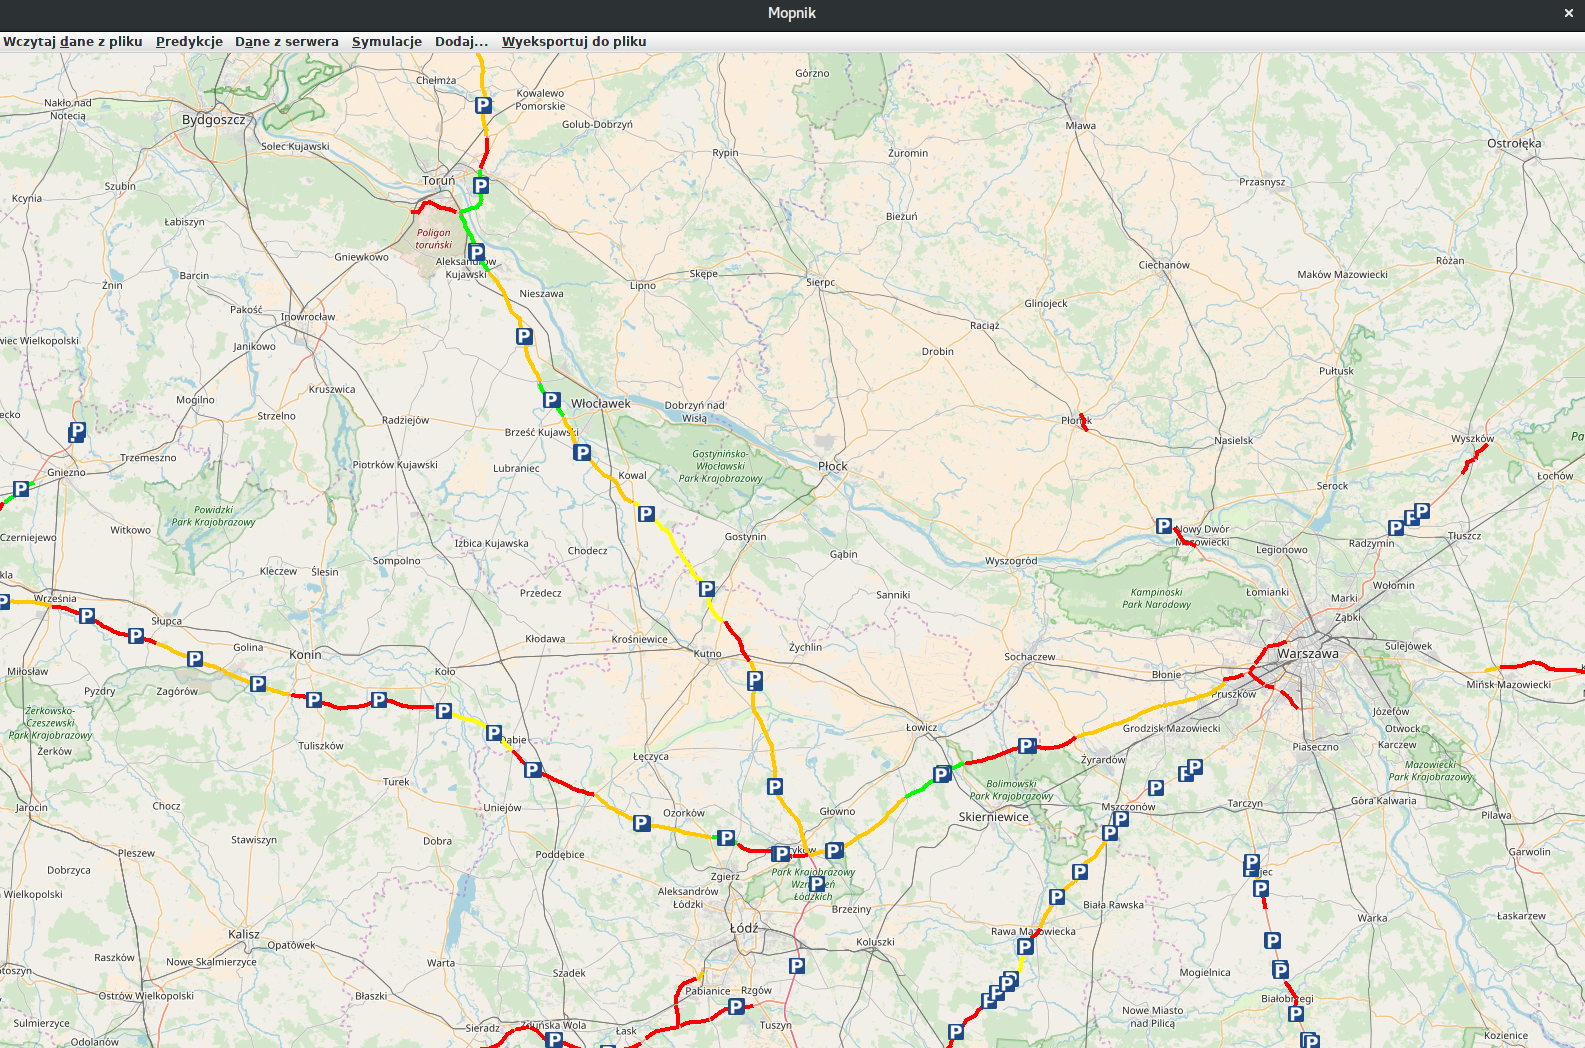
\includegraphics[width=\textwidth]{widok_glowny.png}
      \caption{Widok główny po uruchomieniu programu}
    \end {figure}
    
    Oprócz tego domyślnie jest ustawiona metodyka przewidywania potrzebnych
    miejsc parkingowych pochodząca z pracy Malwiny Spławińskiej i Katarzyny
    Soleckiej
    \footnote{\url{http://www.autobusy-test.com.pl/images/stories/Do_pobrania/2017/nr\%2012/Bezp\%20i\%20ekol/073_013_A_BiE_SPLAWINSKA_SOLECKA.pdf}}.
        Wraz z parametrami zaproponowanymi w tej metodyce.

    Na podstawie tych danych, dla poszczególnych odcinków dróg (ekspresowych i
    autostrad) są wyliczane istniejące oraz potrzebne liczby miejsc
    parkingowych. Są one zaznaczane na mapie kolorami w następujący sposób:
    \begin{itemize}
      \item Kolorem zielonym są zaznaczone te odcinki, gdzie liczba miejsc
        parkingowych jest wystarczająca, a dla niektórych typów pojazdów nawet
        zbyt wysoka.
      \item Kolorem żółtym są zaznaczone te odcinki, gdzie liczba miejsc jest
        wystarczająca (tzn. liczba miejsc wg. metodyki $\ge$ liczba istniejących
        miejsc).
      \item Kolorem pomarańczowym są zaznaczone te odcinki, gdzie brakuje
        miejsc dla pewnego typu pojazdu w co najmniej jednym kierunku.
      \item Kolorem czerwonym są zaznaczone te odcinki, gdzie brakuje miejsca
        dla większości typów pojazdów w obu kierunkach.
     \end{itemize}

        \section{Oglądanie danych}
      Możliwe jest również oglądanie szczegółowych danych dotyczących
      konkretnych MOP-ów oraz konkretnych odcinków sieci drogowej. Po
      kliknięciu w interesującego nas MOP-a lub drogę wyświetla się okno
      dialogowe zawierające m.in. następujące informacje (por. rysunki 2 i 3):
      \begin{itemize}
        \item Dla MOP-a:
          \begin{itemize}
            \item Podstawowe dane takie jak droga, pikietaż, kierunek, oddział.
            \item Liczba miejsc parkingowych dla pojazdów konkretnego typu.
            \item Infrstruktura (stacja bęzynowa, toaleta, restauracja itd.).
          \end{itemize}
        \item Dla odcinka drogi:
          \begin{itemize}
            \item Nazwa drogi oraz pikietaż początku i końca.
            \item Średniodobowe natężenie ruchu na tym odcinku.
            \item Liczba potrzebnych (wg. domyślnej metodyki) oraz liczba
              istniejących w rzeczywistości (suma po MOP-ach stojących przy
              danym odcinku) miejsc parkingowych. Podzielona ze względu na
              kierunek i typ pojazdu.
          \end{itemize}
      \end{itemize}
      \begin{figure}[ht]
        \centering
       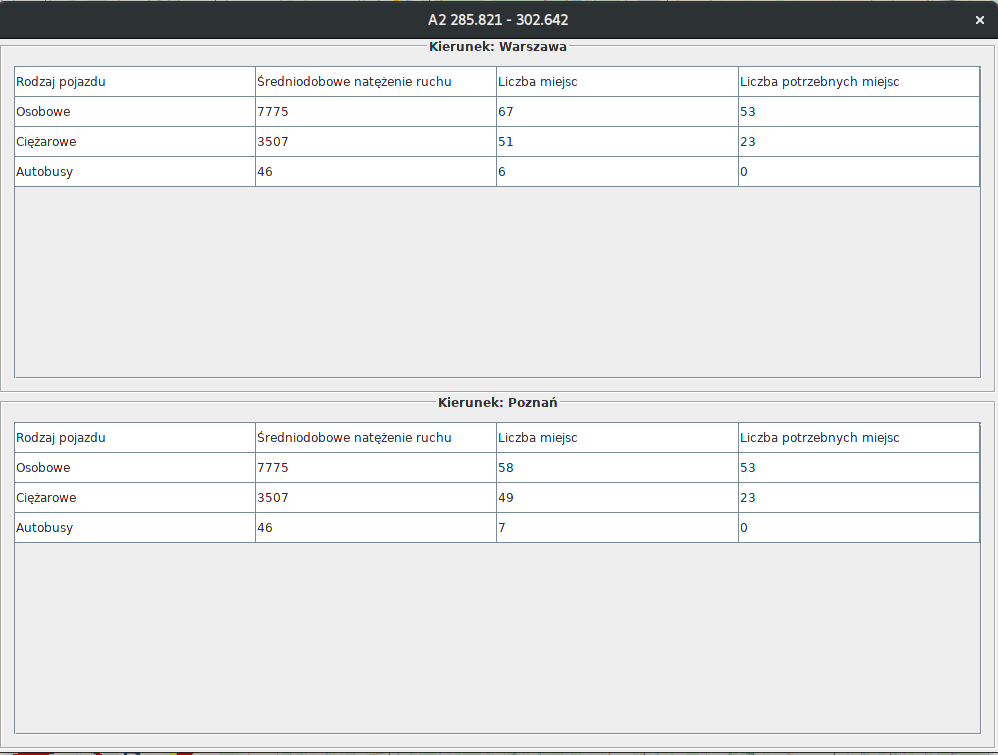
\includegraphics[width=.8\textwidth]{podglad_drogi.png}
        \caption{Podgląd odcinka drogi}
      \end{figure}
      \begin{figure}[ht]
          \centering
          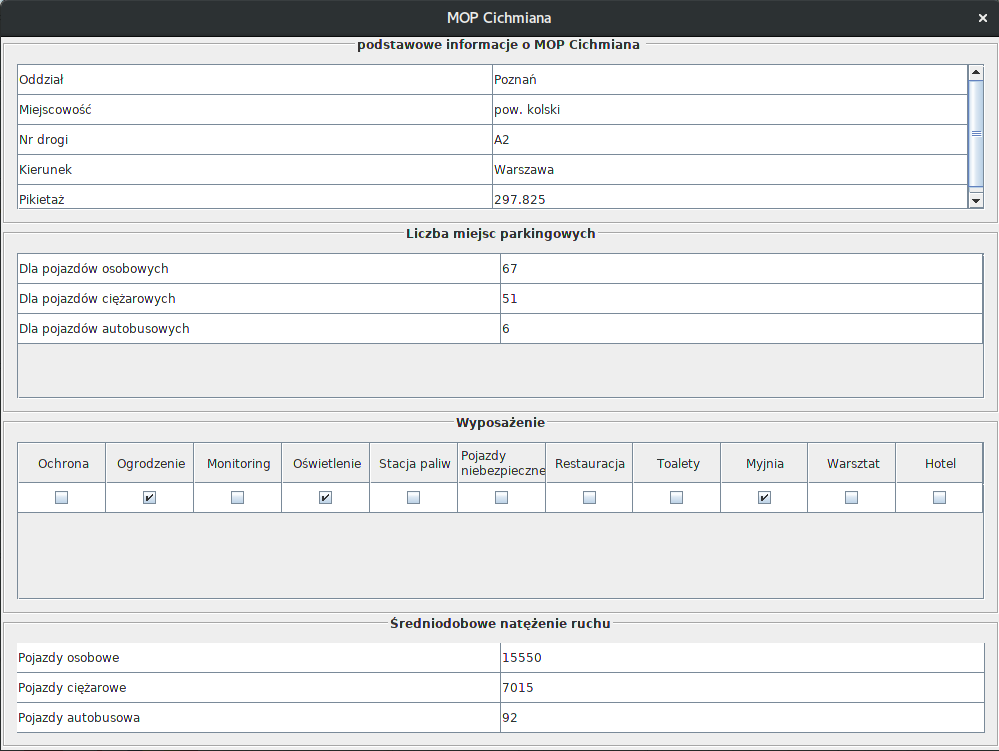
\includegraphics[width=.8\textwidth]{podglad_mopa.png}
          \caption{Podgląd MOP-a}
      \end{figure}

    \chapter{Test Chapter}
    \lipsum[1]

    \section{A Section}
    \lipsum[1]
    
    \chapter{Test Chapter}
    \lipsum[1]
    
    \section{A Section}
    \lipsum[1]

%	\include{multiToC}

    \appendix
    \cleardoublepage\part{Appendix}
    \chapter{Appendix Chapter}
    \lipsum[1]
    
    \section{A Section}
    \lipsum[1]

\end{document}
